% intro
%Les réseaux :
%- [ ] C’est quoi
%- [ ] À quoi ça sert (les enjeux, appliqué)
%- [ ] Quelles sont les questions qui se posent (que dit la recherche)
%
%- [ ] Lauritzen pour les nuls
%
%L’inférence de réseaux :
%- [ ] Quelle méthode pour quel réseau
%- [ ] Auxquelles on se compare, pourquoi elles sont comme ça comment elles marchent et ce qui manque

  \section*{Biological context}
 \subsection*{Networks}
 A network is an intuitive object which anyone can easily relate to. It is first of all a graphical tool representing the links between different entities. This helps understand how a system organizes and have a direct image of it. It is also an analysis tool which can unravel sensible information about the system, its structure and the different roles in its organization. Networks are versatile tools that are  used in many domains (e.g. sociology, linguistics, computer sciences, neurosciences, climatology, psychology, etc.) and can take various forms to adapt to each problem.  They can be directed or undirected. Some link entities with multiple kinds of edges (multidimensional), or have different layers (multiplex), others link groups of disconnected objects (multipartite). In biology, the most typical networks simply represent the species (nodes) and their relationships (edges).

Various types of species interactions are studied with networks. For example, their is a rich literature of networks for plant-pollinator and host-parasite relationships in ecology. These species interactions are clearly defined and directly observed in the field. Contacts of pollination or parasitism are counted and networks constructed from these interaction abundances.
\begin{figure}
\centering
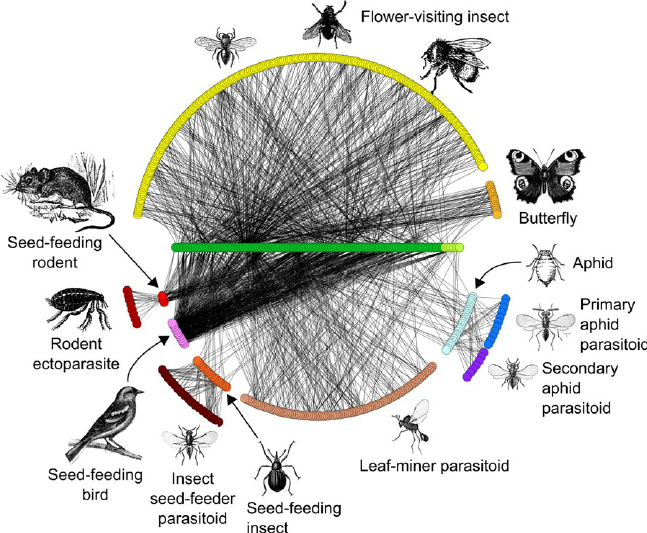
\includegraphics[width=0.7\linewidth]{figs/pocock.png}
\caption{Species interaction networks at Norwood Farm, Somerset, UK \citep{PED12,BRM13}.}
\label{pocock}
\end{figure}
 However many mechanisms cannot be observed and may not be well defined. One way to discover them may then be to resort to a more mathematical definition of species interactions. Working with the latter allows the study of community assembly mechanisms with the inference of networks representing guilds of species in community ecology. This type of network is extensively used in genomics for protein-protein interaction network, or gene regulatory networks, or in microbiology to study the output of a metabarcoding experiment assessing the composition of a microbiome. 
 
 \begin{figure}
\centering
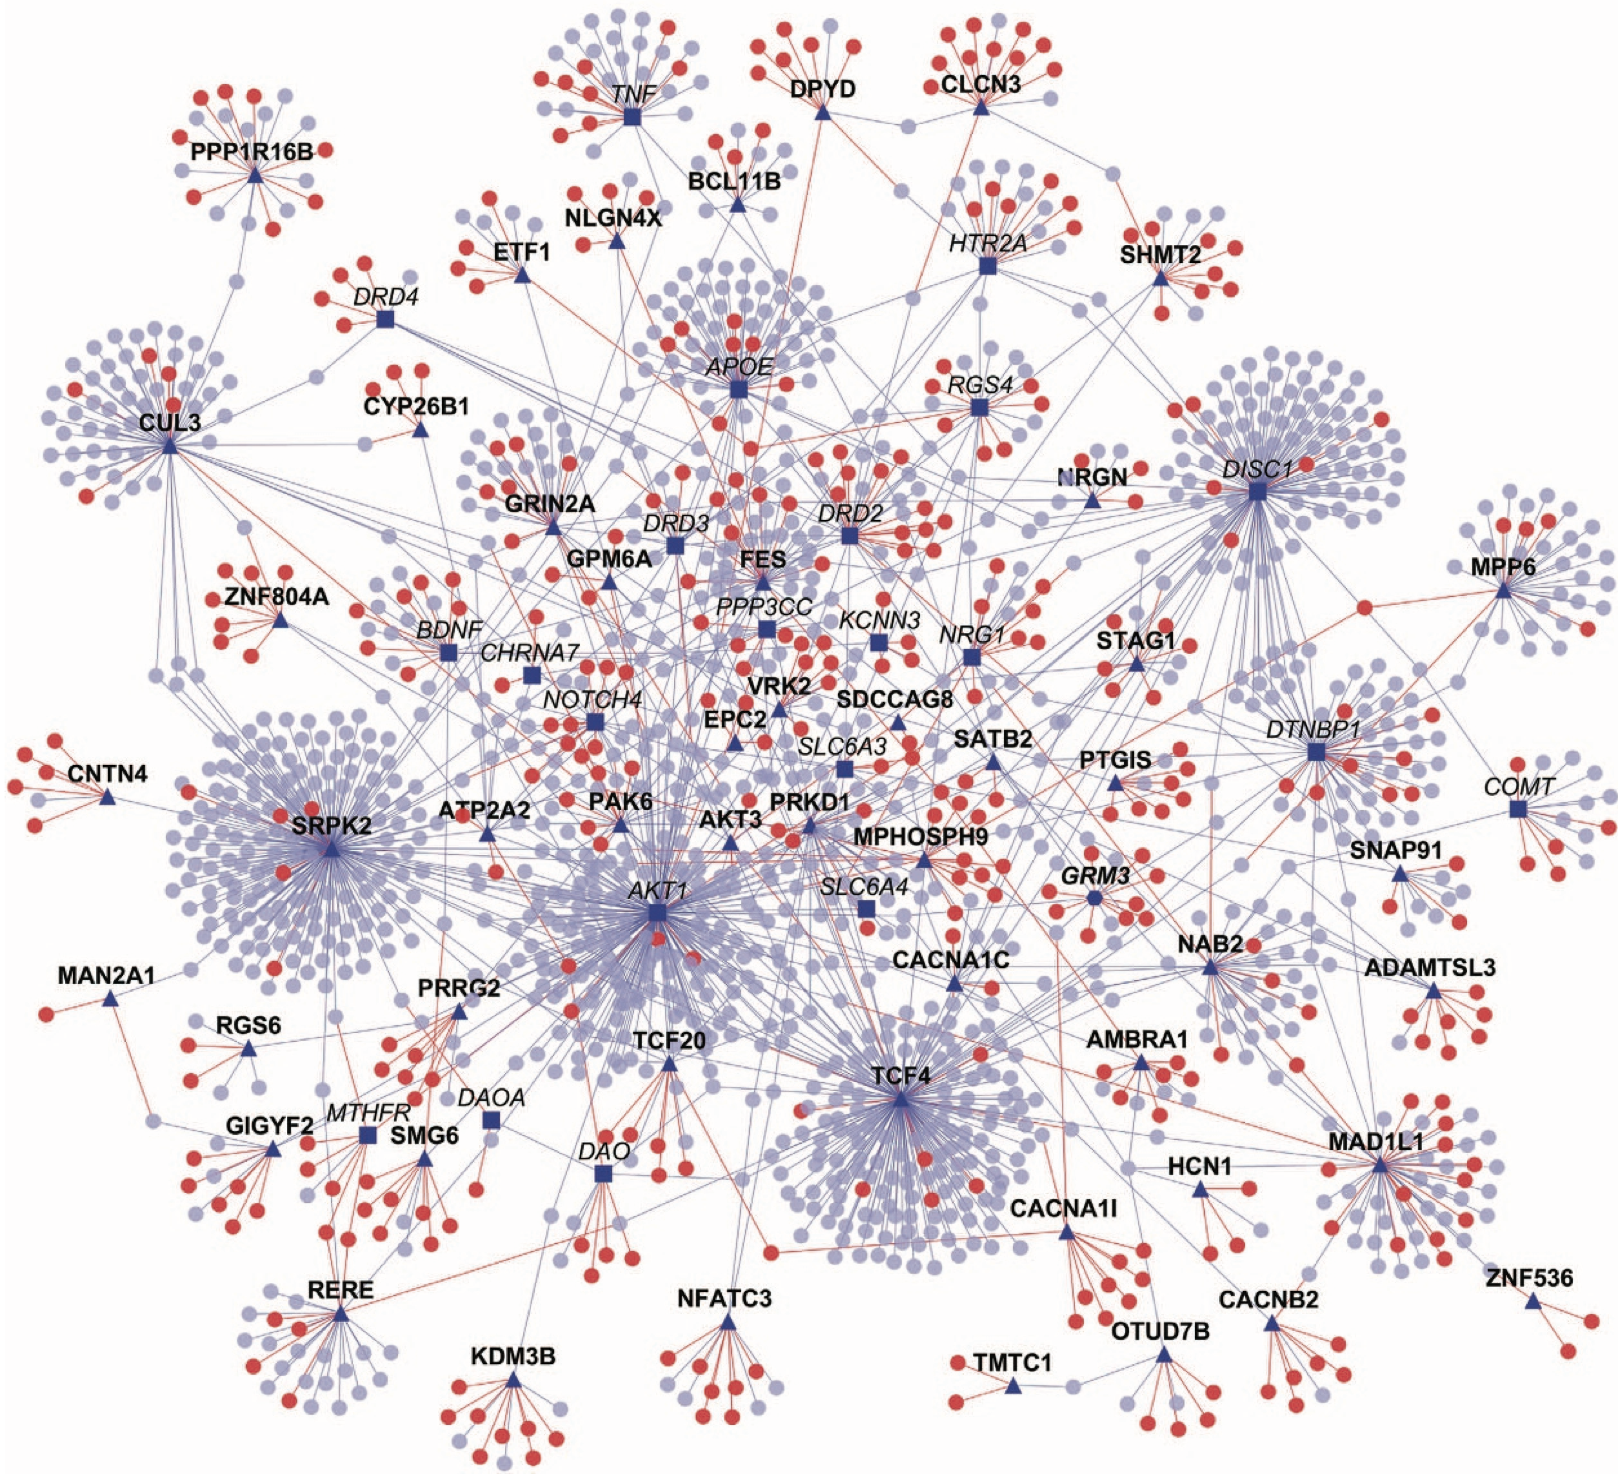
\includegraphics[width=0.7\linewidth]{figs/PPInetwork.png}
\caption{Protein-protein interactions between genes involved in schizophrenia \citep{GTH16}.}
\label{PPI}
\end{figure}

  \subsection*{Statistical interactions}
The correlations between the species measures first come to mind as a statistical characterization of an interaction. These are easily obtained, yet their corresponding networks are hard to interpret. Indeed, two covariates correlating with a same third one will appear correlated, even if they have no direct effect on each other\footnote{e.g. the number of covid 19 cases detected correlates with both the real number of cases and the number of tests done on the population, which induces a spurious correlation between the two latter where obviously there is no direct effect of one on the other.}. This phenomena of spurious correlations complicates both the analysis and the interpretation by inducing a very high number of edges  which cannot be categorized as direct or indirect associations between the species. 
 
 Conditional dependencies are then very useful measures of interaction. They describe dependencies between each pair of species conditional on all others. That is, all other species measures kept fixed, their measures should still be correlated. A link between two species can then be interpreted as a direct association. This yields a network of species conditional dependence (link) and independence (absence of link), which is interpretable and falls within the well-studied mathematical framework of graphical models.
 
 \subsection*{Measures on species}
 Networks of statistical interactions are obtained from datasets of repeated measures on a set of species, which can be of various types. Measures can be continuous, as for example the output of gene expression profiling experiments using DNA microarrays, which  are  fluorescences measures from targeted genes. Using a Gaussian approximation, these measures of genes expressions can be used to derive genes regulatory networks.  Measures can also be binary, as in co-occurrence data in ecology, which record the joint presences and absences of a set of species in several sites. \citet{CAM16}.
%développer les données de co-occurence

Abundance data  are joint counts of species in a series of sites (also known as assemblages data in ecology). Recent technologies made this type of data increasingly available. Assemblages data were rare in ecology as they implied intensive sampling efforts, which is now greatly facilitated by camera traps and sensors. In metagenomics, high-throughput sequencing technologies for metabarcoding experiments made it possible  to get joint counts of pseudo-species (operational taxonomic units (OTUs)) abundances.  Both domains work with the same type of output: a dataset of joint (pseudo-)species abundances from different sites or samples.\\
%développer les metabarcoding et OTU


Once the data has been collected, it is very likely that not all species or covariates were observed: there exists missing actors and data is incomplete. In the network, the existence of a missing actor translates into appearance of edges between all the species it should connect with, creating dense cliques of species which are not actually conditionally dependent on one another. A second objective of this work is to take missing actors into account during network inference in order to get more accurate interpretations.

\section*{Network inference}
% ce qui existe et motivation du sujet
\section*{Objectives}
 \subsection*{Graphical models and Trees}
The dedicated framework for the representation of conditional dependency structures are graphical models. Gaussian Graphical Models (GGM) in particular provide with appealing algebraic properties for network inference, which are detailed in \citet{Lau96}. Exploring the set of possible graphs is a non-ending task, and we chose to reduce the searching space to that of spanning trees. This is the sparsest connected structure, and enjoys specific algebraic properties allowing to sum on all possible spanning trees at the cost of a determinant calculus. Our network inference methodology relies on spanning trees and \citet{Lau96} maximum likelihood estimators for multivariate Gaussian graphical models.

%caser le missing actor qq part
 \subsection*{Modeling abundance data}
 As this ideal framework of GGM is not directly applicable to abundance data, there exist two possible ways to proceed: either apply a Gaussian transformation to the data, or rely on Gaussian latent vectors in the framework of Joint Species Distribution Models (JSDM). Our methodology resorts to the latter, and more specifically to the Poisson log-normal distribution to model the counts. This distribution allows easy handling of both covariates and offsets, as well as take overdispersion into account thanks to its Gaussian random parameters. 
 
 
 \subsection*{Estimation procedure} %or algorithm
The central model we adopt involves a Gaussian layer of parameters which is a mixture on all spanning trees. Each component of the mixture is a Gaussian distribution which dependency structure is a spanning tree. This represents two hidden layers of parameters, which we first estimates with an Estimation-Maximization (EM) algorithm. Then to infer missing actors of the network, we resort to a variational (VEM) approach.

\section*{Outline} 
  \subsection*{Chapter 1}
The first chapter details the mathematical tools and technical results for the statistical modeling and the network inference used in Chapters 2 and 3.

   \subsection*{Chapter 2}
   This chapter details a method to infer undirected networks representing conditional statistical dependencies between the species from their joint abundance measures.  The proposed methodology, implemented in the R package \texttt{EMtree},  is compared to state of the art approaches and applied to two empirical datasets from ecology and metagenomics. This chapter has been published as an article in the journal \textit{Methods in Ecology and Evolution} \citep{MRA20}.
   
    \subsection*{Chapter 3}
This chapter details a variational approach to the inference of a missing actor in the network. The reconstruction of missing actor(s) is implemented in the R package \texttt{nestor} and illustrated on two  empirical datasets from ecology. This chapter has been submitted for publication in the \textit{Journal of the Royal Statistical Society: series C (applied statistics)}.
 
  \subsection*{Chapter 4}
This final chapter introduces some natural perspectives of this work. After concluding on the specifics of the developed methodology, natural extension are presented, including network comparison. The inclusion of spatialized data is discussed, as well as the possibility of network inference directly from the observed counts.
 \section*{Notations}
 
 \begin{description}
 \item[Operations:]  \begin{itemize}
     \item[]
 \item[] $|\cdot|$ : matrix determinant
 \item[] $\odot$ : Hadamard product
 \end{itemize}
 \item[Variables:] \begin{itemize}
     \item[]
 \item[] $\Ybf$ :  matrix  of observed counts
 \item[] $\Zbf$ : matrix of latent Gaussian parameters 
 \item[] $\Ubf$ : matrix of latent normalized Gaussian parameters 
 \item[] $\Xbf$ : matrix of covariates 
 \item[] $O$ : matrix of measured offsets
 \end{itemize}
 \item[Dimensions:]\begin{itemize}
     \item[]
 \item[] $n$ : number of samples
 \item[] $p$: number of observed species
 \item[] $r$: number of unobserved species
 \item[] $d$: number of covariates
 \end{itemize}
 \end{description} 